
\documentclass{article}[14pt]
\usepackage{multicol, enumerate, enumitem, hyperref, color, soul, setspace, parskip, fancyhdr, amssymb, amsthm, amsmath, bbm, latexsym, units, mathtools}
\everymath{\displaystyle}
\usepackage[headsep=0.5cm,headheight=0cm, left=1 in,right= 1 in,top= 1 in,bottom= 1 in]{geometry}
\pagestyle{fancy}
\lhead{}
\chead{Answer Key for Module\,6\,-\,Polynomial\,Functions Version C}
\rhead{}
\lfoot{Summer\,C\,2020}
\cfoot{}
\rfoot{}
\begin{document}
\textbf{This key should allow you to understand why you choose the option you did (beyond just getting a question right or wrong). \href{https://xronos.clas.ufl.edu/mac1105spring2020/courseDescriptionAndMisc/Exams/LearningFromResults}{More instructions on how to use this key can be found here}.}

\textbf{If you have a suggestion to make the keys better, \href{https://forms.gle/CZkbZmPbC9XALEE88}{please fill out the short survey here}.}

\textit{Note: This key is auto-generated and may contain issues and/or errors. The keys are reviewed after each exam to ensure grading is done accurately. If there are issues (like duplicate options), they are noted in the offline gradebook. The keys are a work-in-progress to give students as many resources to improve as possible.}

\rule{\textwidth}{0.4pt}

26. Which of the following equations \textit{could} be of the graph presented below?
\begin{center} 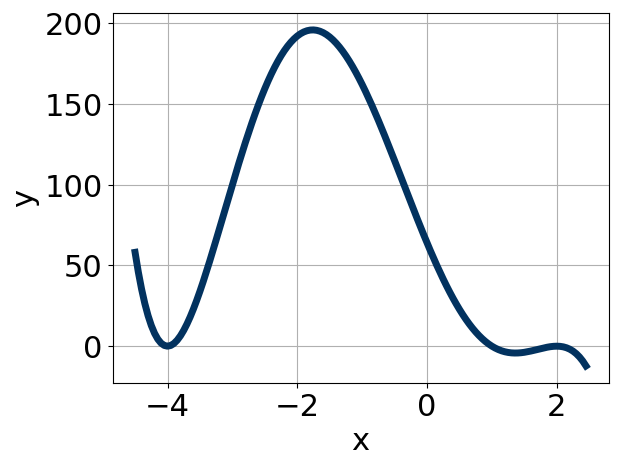
\includegraphics[width=0.3\textwidth]{../Figures/polyGraphToFunctionC.png} \end{center} 

The solution is $ -2x^{8} (x + 1)^{8} (x + 2)^{4} $ 

\begin{enumerate}[label=\Alph*.] 
\item $ -18x^{10} (x + 1)^{9} (x + 2)^{5} $ 

 The factors $(x + 1)$ and $(x + 2)$ should both have even powers. 
\item $ -8x^{6} (x + 1)^{10} (x + 2)^{11} $ 

 The factor $(x + 2)$ should have an even power. 
\item $ -2x^{8} (x + 1)^{8} (x + 2)^{4} $ 

 * This is the correct option. 
\item $ 6x^{4} (x + 1)^{10} (x + 2)^{9} $ 

 The factor $(x + 2)$ should have an even power and the leading coefficient should be the opposite sign. 
\item $ 14x^{4} (x + 1)^{8} (x + 2)^{4} $ 

 This corresponds to the leading coefficient being the opposite value than it should be. 
\end{enumerate} 
 
General Comments: Draw the x-axis to determine which zeros are touching (and so have even multiplicity) or cross (and have odd multiplicity).

-----------------------------------------------

27. Construct the lowest-degree polynomial given the zeros below. Then, choose the intervals that contain the coefficients of the polynomial in the form $x^3+bx^2+cx+d$.
$$ -4 + 2i \text{ and } -3 $$ 
The solution is $ x^{3} +11 x^{2} +44 x + 60 $ 

\begin{enumerate}[label=\Alph*.] 
\item $ b \in [0, 6], c \in [-3, 5], \text{ and } d \in [-10, -3] $ 

 $x^{3} + x^{2} +x -6$, which corresponds to multiplying out $(x -2)(x + 3)$. 
\item $ b \in [0, 6], c \in [5, 12], \text{ and } d \in [9, 14] $ 

 $x^{3} + x^{2} +7 x + 12$, which corresponds to multiplying out $(x + 4)(x + 3)$. 
\item $ b \in [5, 12], c \in [43, 55], \text{ and } d \in [51, 63] $ 

 * $x^{3} +11 x^{2} +44 x + 60$, which is the correct option. 
\item $ b \in [-16, -9], c \in [43, 55], \text{ and } d \in [-67, -56] $ 

 $x^{3} -11 x^{2} +44 x -60$, which corresponds to multiplying out $(x-(-4 + 2i))(x-(-4 - 2i))(x -3)$. 
\item $ \text{None of the above.} $ 

 This corresponds to making an unanticipated error or not understanding how to use nonreal complex numbers to create the lowest-degree polynomial. If you chose this and are not sure what you did wrong, please contact the coordinator for help. 
\end{enumerate} 
 
General Comments: Remember that the conjugate of $a+bi$ is $a-bi$. Since these zeros always come in pairs, we need to multiply out $(x-(-4 + 2i))(x-(-4 - 2i))(x-(-3))$.

-----------------------------------------------

28. Construct the lowest-degree polynomial given the zeros below. Then, choose the intervals that contain the coefficients of the polynomial in the form $ax^3+bx^2+cx+d$.
$$ \frac{1}{4}, -5, \text{ and } 7 $$ 
The solution is $ 4x^{3} -9 x^{2} -138 x + 35 $ 

\begin{enumerate}[label=\Alph*.] 
\item $ a \in [0, 7], b \in [-47.7, -42], c \in [120, 137], \text{ and } d \in [31, 41] $ 

 $4x^{3} -47 x^{2} +128 x + 35$, which corresponds to multiplying out $(4x + 4)(x + 1)(x -1)$. 
\item $ a \in [0, 7], b \in [-12.1, -7.8], c \in [-139, -134], \text{ and } d \in [-43, -30] $ 

 $4x^{3} -9 x^{2} -138 x -35$, which corresponds to multiplying everything correctly except the constant term. 
\item $ a \in [0, 7], b \in [-12.1, -7.8], c \in [-139, -134], \text{ and } d \in [31, 41] $ 

 * $4x^{3} -9 x^{2} -138 x + 35$, which is the correct option. 
\item $ a \in [0, 7], b \in [-8.9, -6.8], c \in [-149, -141], \text{ and } d \in [-43, -30] $ 

 $4x^{3} -7 x^{2} -142 x -35$, which corresponds to multiplying out $(4x + 4)(x -1)(x -1)$. 
\item $ a \in [0, 7], b \in [8.2, 12.2], c \in [-139, -134], \text{ and } d \in [-43, -30] $ 

 $4x^{3} +9 x^{2} -138 x -35$, which corresponds to multiplying out $(4x + 1)(x -5)(x + 7)$. 
\end{enumerate} 
 
General Comments: To construct the lowest-degree polynomial, you want to multiply out $(4x -1)(x + 5)(x -7)$

-----------------------------------------------

29. Describe the end behavior of the polynomial below.
$$ f(x) = 8(x - 7)^{5}(x + 7)^{10}(x + 8)^{5}(x - 8)^{5} $$ 

 
 The solution is  
 \begin{center} 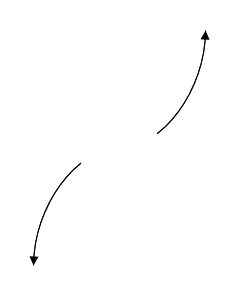
\includegraphics[width=0.3\textwidth]{../Figures/endBehaviorPositiveOddC.png} \end{center}\begin{tabular}{|c|c|} 
\hline 
 & \tabularnewline 
 \textbf{A.} 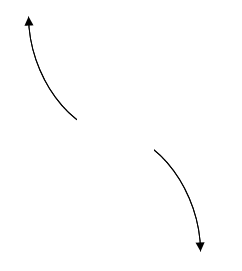
\includegraphics[width=0.3\textwidth]{../Figures/endBehaviorNegativeOddC.png} & \textbf{B.} 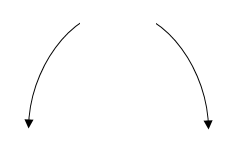
\includegraphics[width=0.3\textwidth]{../Figures/endBehaviorNegativeEvenC.png} \tabularnewline 
\hline 
 & \tabularnewline 
 \textbf{C.} 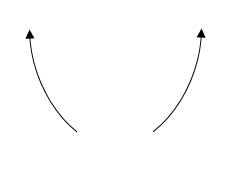
\includegraphics[width=0.3\textwidth]{../Figures/endBehaviorPositiveEvenC.png} & \textbf{D.} 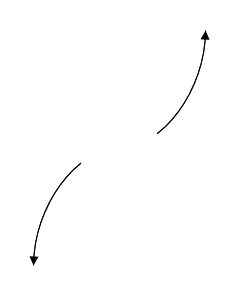
\includegraphics[width=0.3\textwidth]{../Figures/endBehaviorPositiveOddC.png} \tabularnewline 
\hline 
 E. None of the figures above. & \tabularnewline 
\hline 
 \end{tabular} 
 
\textbf{General Comments:} Remember that end behavior is determined by the leading coefficient AND whether the \textbf{sum} of the multiplicities is positive or negative.

-----------------------------------------------

30. Describe the zero behavior of the zero $x = -4$ of the polynomial below.
$$ f(x) = -9(x - 7)^{6}(x + 7)^{3}(x - 4)^{10}(x + 4)^{7} $$ 

 
 The solution is  
 \begin{center} 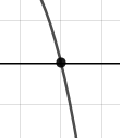
\includegraphics[width=0.3\textwidth]{../Figures/zeroBehaviorNegativeOddC.png} \end{center}\begin{tabular}{|c|c|} 
\hline 
 & \tabularnewline 
 \textbf{A.} 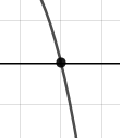
\includegraphics[width=0.3\textwidth]{../Figures/zeroBehaviorNegativeOddC.png} & \textbf{B.} 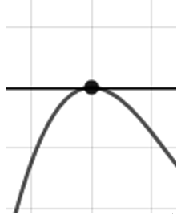
\includegraphics[width=0.3\textwidth]{../Figures/zeroBehaviorNegativeEvenC.png} \tabularnewline 
\hline 
 & \tabularnewline 
 \textbf{C.} 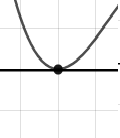
\includegraphics[width=0.3\textwidth]{../Figures/zeroBehaviorPositiveEvenC.png} & \textbf{D.} 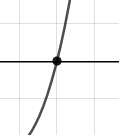
\includegraphics[width=0.3\textwidth]{../Figures/zeroBehaviorPositiveOddC.png} \tabularnewline 
\hline 
 E. None of the figures above. & \tabularnewline 
\hline 
 \end{tabular} 
 
\textbf{General Comments:} You will need to sketch the entire graph, then zoom in on the zero the question asks about.

-----------------------------------------------


\end{document}

